%!TEX root = ../../thesis.tex

\ac{EW} theory contains several free parameters that must be experimentally 
determined: five couplings ($g$, $g'$, $g_{\Pe}$, $g_{\Pmu}$, $g_{\Ptau}$) and two 
Higgs sector parameters ($\mu$, $\lambda$). Using relations from \Section~\ref{sec:ewsb},
it is advantageous to choose an alternative set of independent parameters more closely
connected to experiment: $\alpha$, \mW, \mZ, \mH, $m_{\Pe}$, $m_{\Pmu}$, $m_{\Ptau}$.
Finding the Higgs boson and measuring its mass was therefore of fundamental importance to 
understanding the \ac{EW} sector, and this was a primary goal of the \ac{LHC}. 

Prior to the \ac{LHC}, the value of \mH was constrained through theoretical 
considerations, direct searches at previous colliders and global fits of other 
electroweak observables.



\subsection{Theoretical constraints}
\label{sec:prior_constraints:theory}

Like all coupling constants in a renormalisable theory, the Higgs quartic coupling 
$\lambda$ `runs' with energy scale $\Lambda$, as described by the \acp{RGE}. The running 
is characterised by the $\beta$-function:
\begin{equation*}
	\beta_{\lambda} = \frac{\partial \lambda}{\partial \log\Lambda}
\end{equation*}

For high \mH, self-couplings dominate $\beta_{\lambda}$, which have a
positive contribution. Therefore $\lambda$ increases with the scale, and above some 
critical scale $\Lambda_c$ the \ac{EW} theory is no longer perturbative. Thus we would 
either expect to observe non-perturbative behaviour at scales \about$\Lambda_c$ or new 
physics at a scale $<\Lambda_c$ that circumvents this issue. Larger values of \mH lead to 
lower values of $\Lambda_c$ and are therefore disfavoured (blue line in 
\Figure~\ref{fig:theory_constraints}). Requiring perturbativity up to the 
reduced Planck scale of \unit{$\Lambda_{P} \about 10^{18}$}{\GeV} (where we expect new 
physics describing gravity) places an upper bound on \mH of \unit{175}{\GeV} 
\cite{Ellis:2009}.

For small \mH, top loops dominate $\beta_{\lambda}$, which have a negative 
contribution. Therefore $\lambda$ decreases as the scale increases, and above some 
critical scale $\Lambda_c$ the coupling becomes negative. At such scales, the \ac{EW} 
vacuum is simply a local minimum and it is possible for the Universe to collapse through
quantum tunnelling into the more stable vacuum state (green band in 
\Figure~\ref{fig:theory_constraints}). Requiring vacuum stability up to $\Lambda_{P}$ 
places a lower bound on \mH of \unit{129}{\GeV} \cite{Ellis:2009}. It is also possible 
to consider a metastable Universe whose expected lifetime is longer than its age.
Accounting for thermal fluctuations up to temperatures \about $\Lambda_{P}$, the \ac{EW}
vacuum has a sufficiently long lifetime if \unit{\mH$>$122}{\GeV} (pale blue band in 
\Figure~\ref{fig:theory_constraints}) \cite{Ellis:2009}. These bounds are rather 
sensitive to the top mass, which has a large uncertainty.

\begin{figure}
	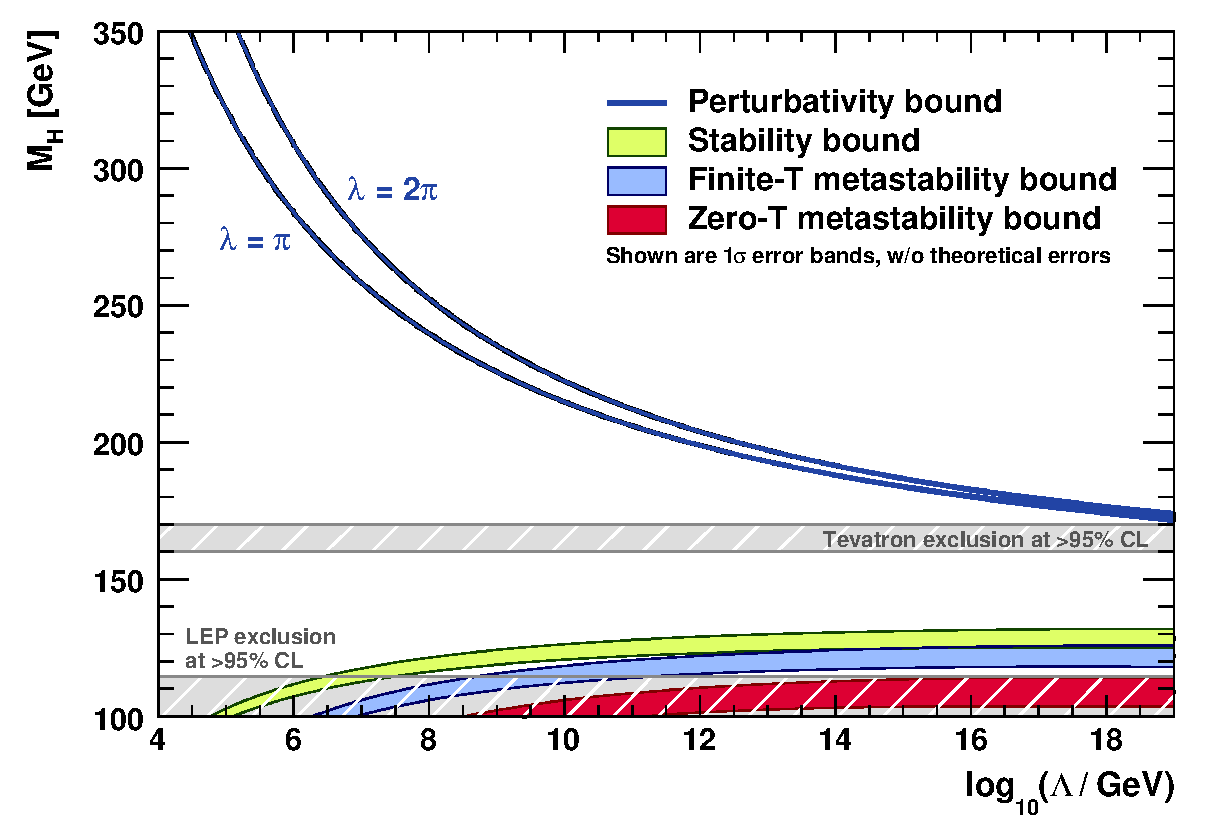
\includegraphics[width=\mediumfigwidth]{tex/motivation/theory_constraints}
	\caption{The scale $\Lambda$ at which the Higgs quartic coupling becomes 
	non-perturbative (blue lines) or an instability in the \ac{EW} vacuum appears
	(green band) \cite{Ellis:2009}. The two blue lines represent different degrees of 
	non-perturbativity (lower line corresponds to a two-loop correction of 25\%, upper 
	line is 50\%), and their difference is indicative of the theoretical uncertainty in 
	this bound. The blue and red bands are bounds for a metastable Universe including and
	neglecting thermal fluctuations respectively.}
	\label{fig:theory_constraints}
\end{figure}



\subsection{Direct searches}
\label{sec:prior_constraints:direct}

Experimental searches for the Higgs boson were first performed at LEP (CERN, Geneva), which ran from 1989 to 2000. This was a circular \epluseminus collider with a \ac{CM} 
energy tuned to the \PZ-pole and then varied between 189 and \unit{209}{\GeV}. A combined 
search for \ZH was performed using an integrated luminosity of \unit{2.5}{\invfb}, which 
excluded \mH $<$ \unit{114.4}{\GeV} at the 95\% \ac{CL} \cite{LEP:2003}.

Further searches were performed at the Tevatron (FNAL, Illinois), which ran from 1987
to 2011. This was a circular \ppbar collider with \ac{CM} energies of \unit{1.8}{\TeV}
and \unit{1.96}{\TeV}. Searches using a variety of production and decay modes were
combined across experiments using datasets corresponding to integrated luminosities up to
\unit{12.6}{\invfb}. Higgs masses below \unit{109}{\GeV} and between 158 and 
\unit{175}{\GeV} were excluded at the 95\% \ac{CL} \cite{Tevatron:2010}.

% \begin{figure}
% 	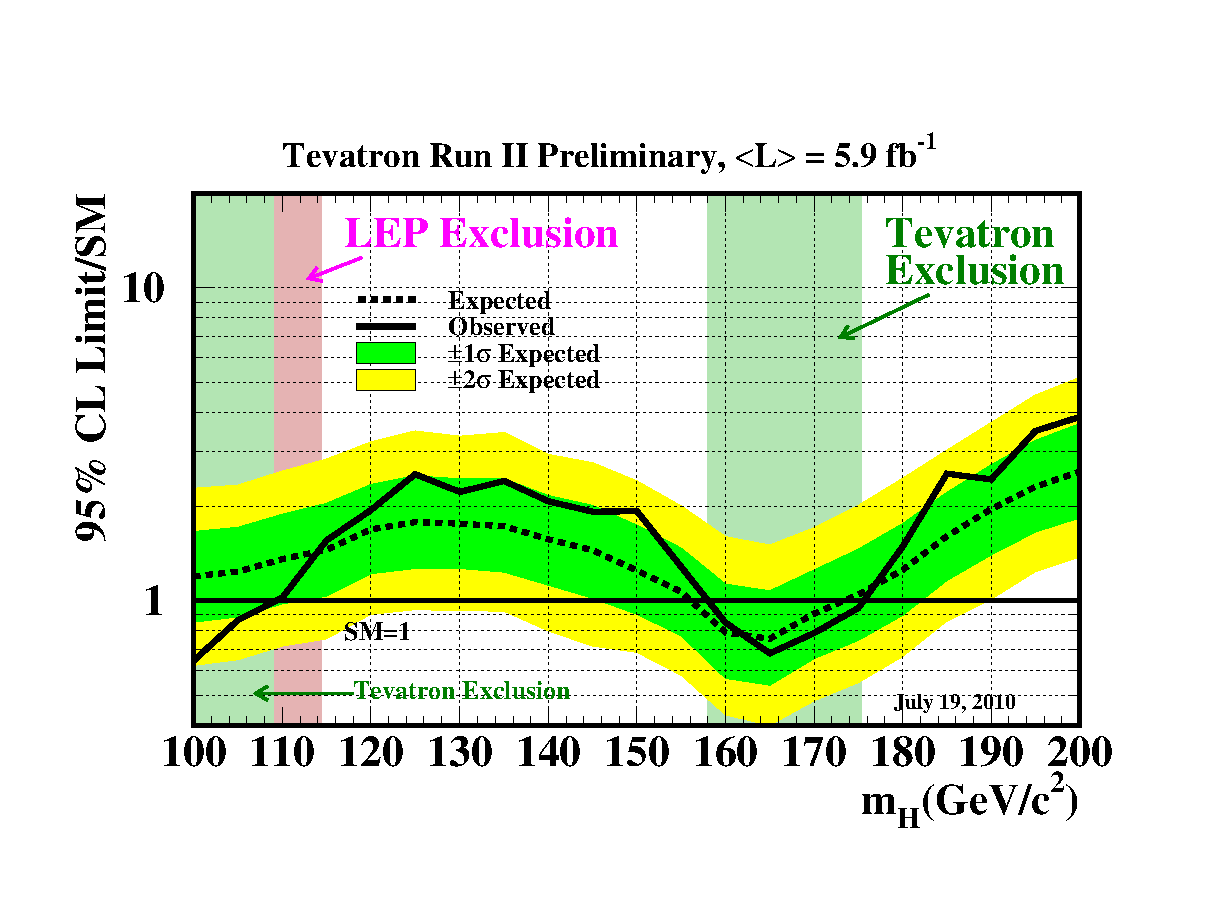
\includegraphics[width=\mediumfigwidth]{tex/motivation/tevatron_limit}
% 	\caption{Observed and expected 95\% \ac{CL} upper limits on the ratio to the \ac{SM} 
% 	cross section versus \mH, obtained through combination of multiple CDF and \dzero 
% 	analyses \cite{Tevatron:2010}. The analyses use datasets corresponding to integrated 
% 	luminosities up to \unit{5.9}{\invfb} at CDF and up to \unit{6.7}{\invfb} at \dzero.}
% 	\label{fig:existing_limits}
% \end{figure}



\subsection{Precision electroweak fits}
\label{sec:prior_constraints:ew_fits}

The \ac{SM} predicts that many observables will depend upon \mH through loop corrections,
and it is therefore possible to infer \mH through precision \ac{EW} measurements. Since 
the leading \mH dependence is logarithmic, the inferred constraints are weaker than those
used to predict the top mass (where the dependence is quadratic).

Performing a global fit of various electroweak measurements at the \ac{LEP}, SLC and
Tevatron colliders (\eg \mW, $\Gamma_{\PW}$, $m_{\Ptop}$), it was possible to exclude 
\mH$>$\unit{158}{\GeV} at the 95\% \ac{CL} \cite{Gfitter:2008}. However, the best fit \mH
was excluded by direct searches, as shown in \Figure~\ref{fig:ewfit}.

\begin{figure}
	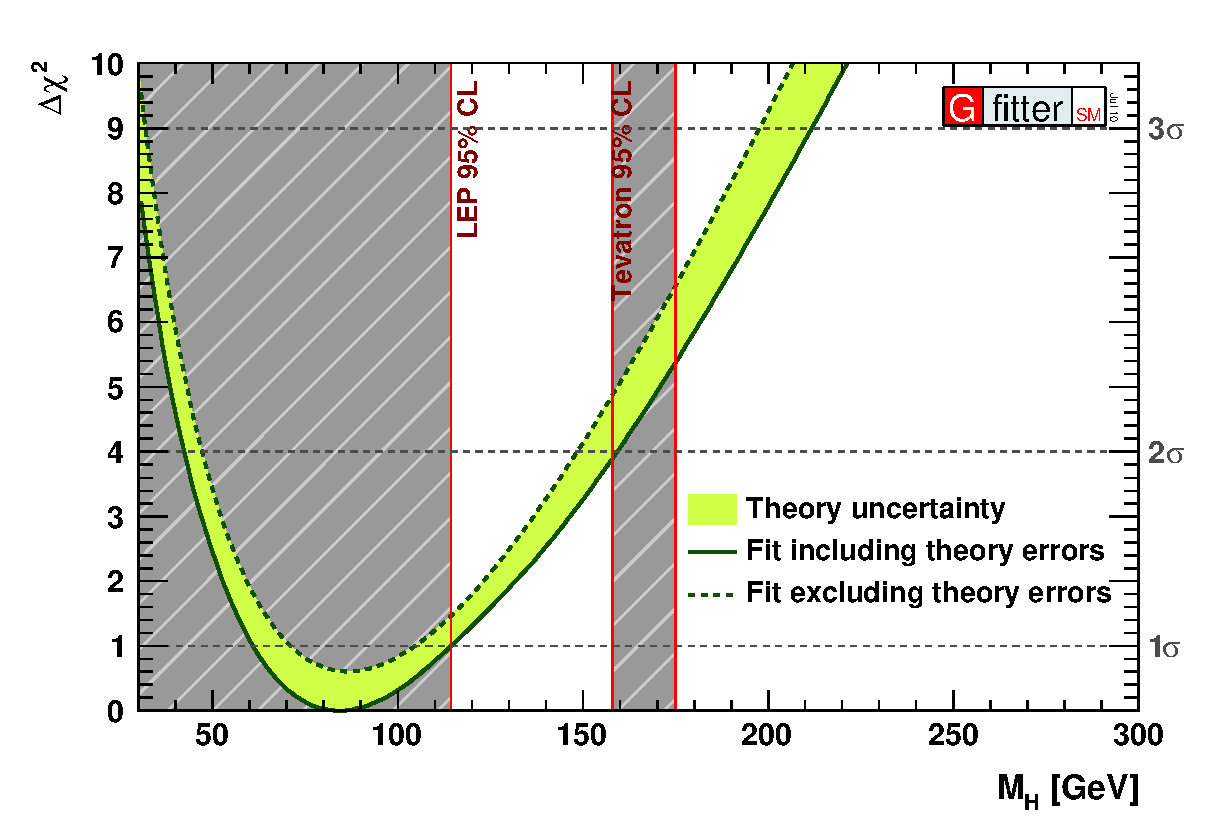
\includegraphics[width=0.495\textwidth]{tex/motivation/ewfit_nodirect}
	\hfill
	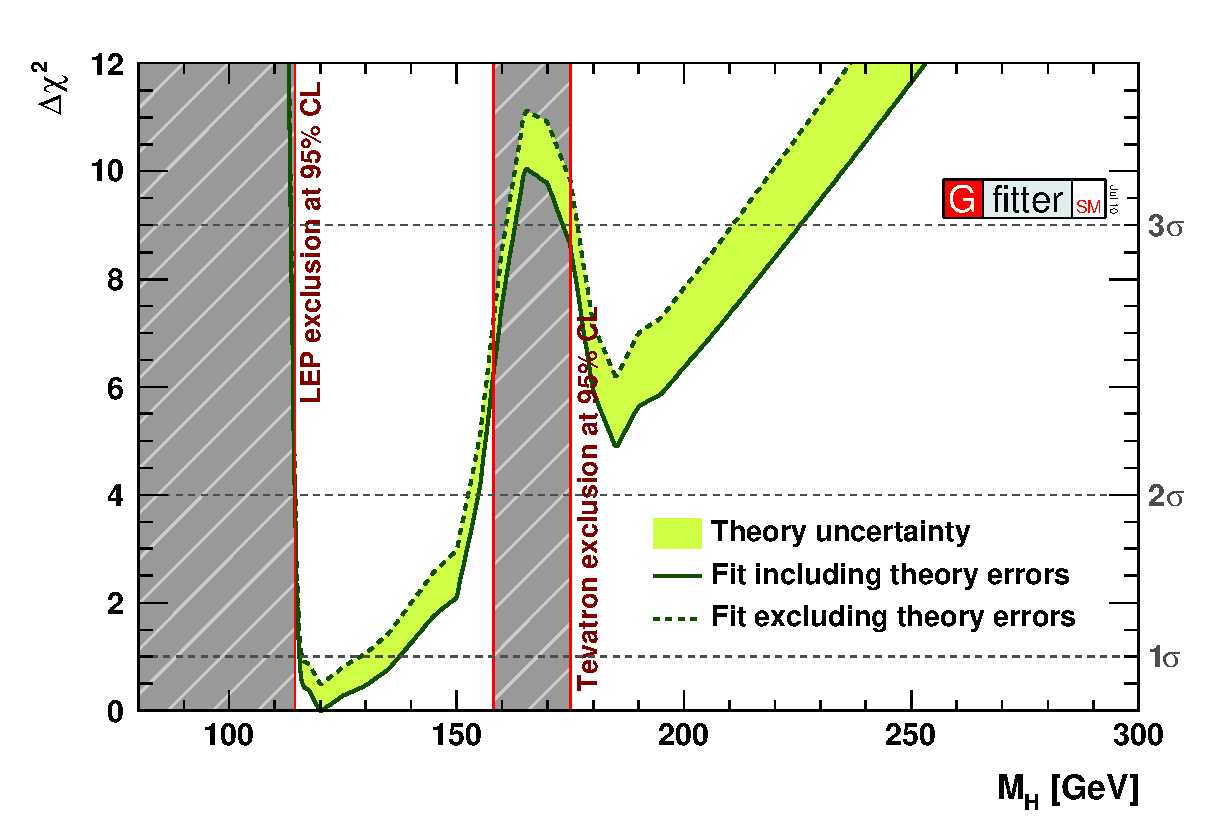
\includegraphics[width=0.495\textwidth]{tex/motivation/ewfit_withdirect}
	\caption{The observed $\Delta\chi^2 = \chi^2 - \chi^2_{\min}$ of electroweak fits 
	versus \mH, neglecting (left) and including (right) results from direct searches
	\cite{Gfitter:2008}. The exclusion limits from LEP and the Tevatron are also shown.}
	\label{fig:ewfit}
\end{figure}

% \begin{figure}
% 	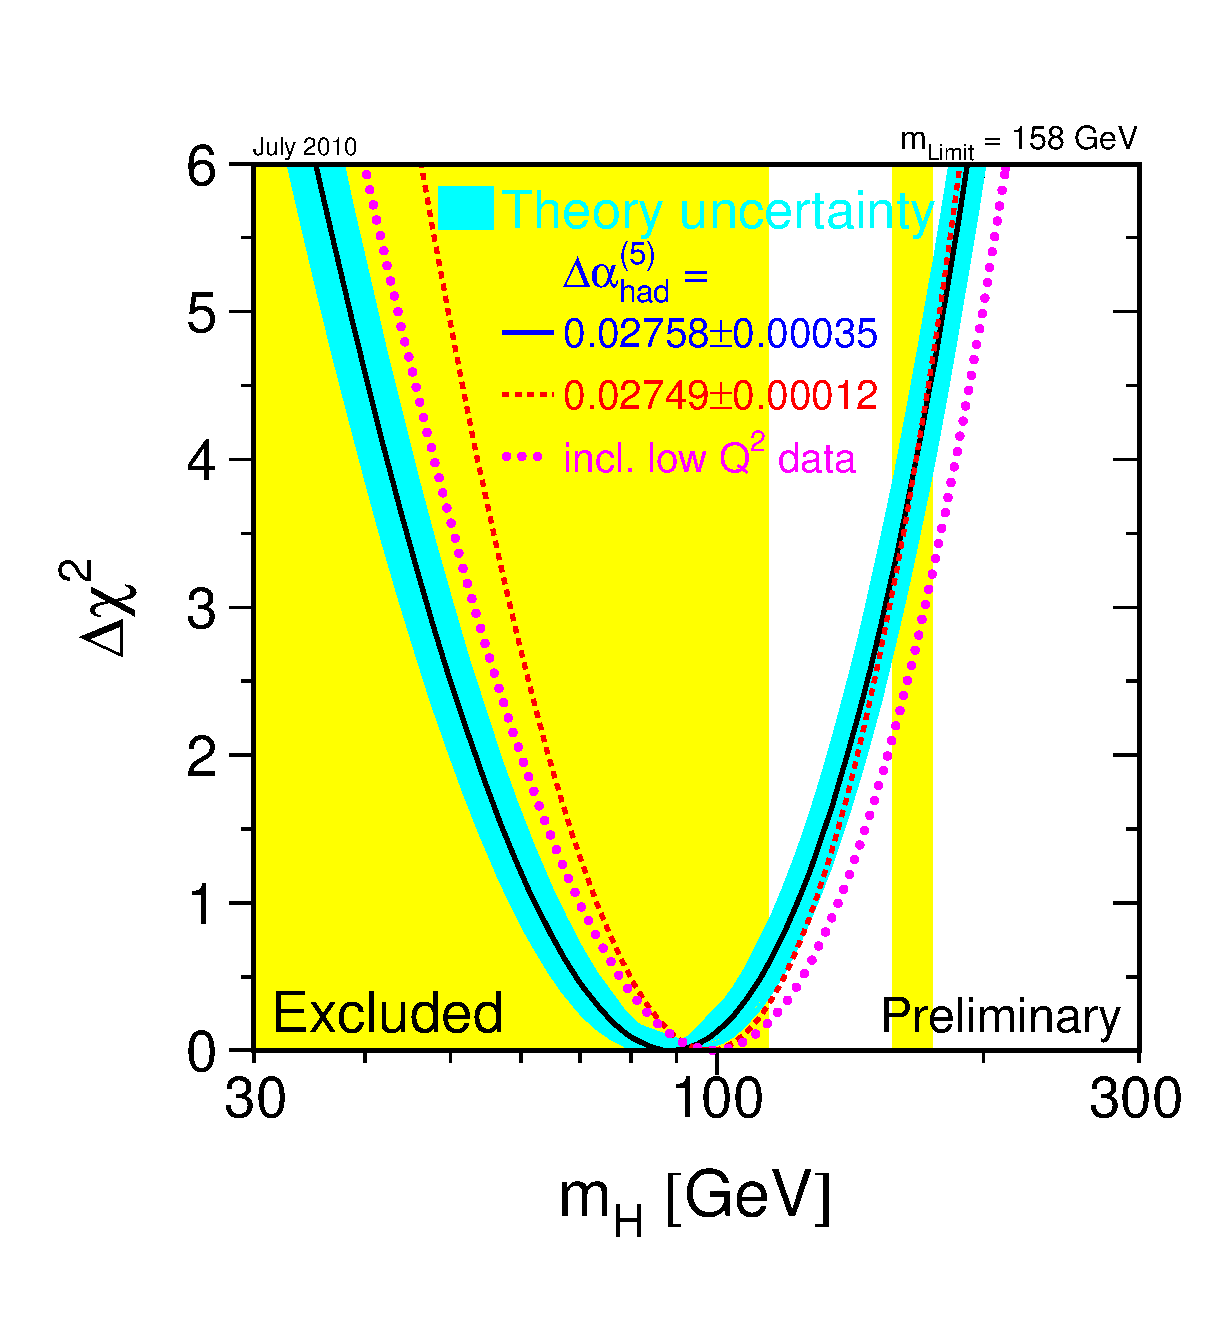
\includegraphics[width=\mediumfigwidth]{tex/motivation/ew_fit_chi2}
% 	\caption{The observed $\Delta\chi^2 = \chi^2 - \chi^2_{\min}$ of electroweak fits 
% 	versus \mH \cite{Grunewald:2010}. The line is fit using \PZ-pole data and direct 
% 	measurements of \mW, $\Gamma_{\PW}$ and $m_{\Ptop}$, and the band is an estimate of 
% 	the uncertainty due to missing higher order corrections. The dashed line uses an 
% 	alternative value of the hadronic vacuum polarisation to show the effect of 
% 	uncertainty in $\alpha(m_{\PZ}^2)$. The dotted line includes low-$Q^2$ experimental 
% 	data. The vertical bands show the 95\% \ac{CL} exclusion limits on \mH arising from 
% 	direct searches at the \ac{LEP} and the Tevatron.}
% 	\label{fig:ewfit}
% \end{figure}
